\subsubsection{Cerca en Profunditat (DFS)}

Com hem mencionat, aquest algorisme comença amb un node inicial, i continua per tots els altres nodes als quals es pot accedir des d'aquest node mitjançant les arestes del graf.

La cerca en profunditat sempre recorre un mateix camí, metres que hi hagi més nodes que no hàgem visitat i adjacents al node en el qual ens situem.

Quan això no es compleix, tornem als nodes anteriors i a partir d'aquests tornem a explorar fins que de nou no hi han més nodes no visitats adjacents al node en el qual ens situem, de nou tornem als nodes anteriors i així successivament fins que ja hem explorat tots els nodes que podíem explorar des del node inicial, cal recalcar que l'algorisme té control dels nodes que ja han estat visitats, de manera que processa un node tan sols una vegada, si no ho féssim així, podríem trobar-nos en un bucle infinit on anem d'un node A fins a un node B i a la inversa successivament fins a l'infinit.

Cal recalcar que la complexitat temporal de l'algorisme DFS és de $O(n+m)$ on $n$ representa el nombre de nodes i $m$ el nombre d'arestes en tot el graf.

\begin{center}
    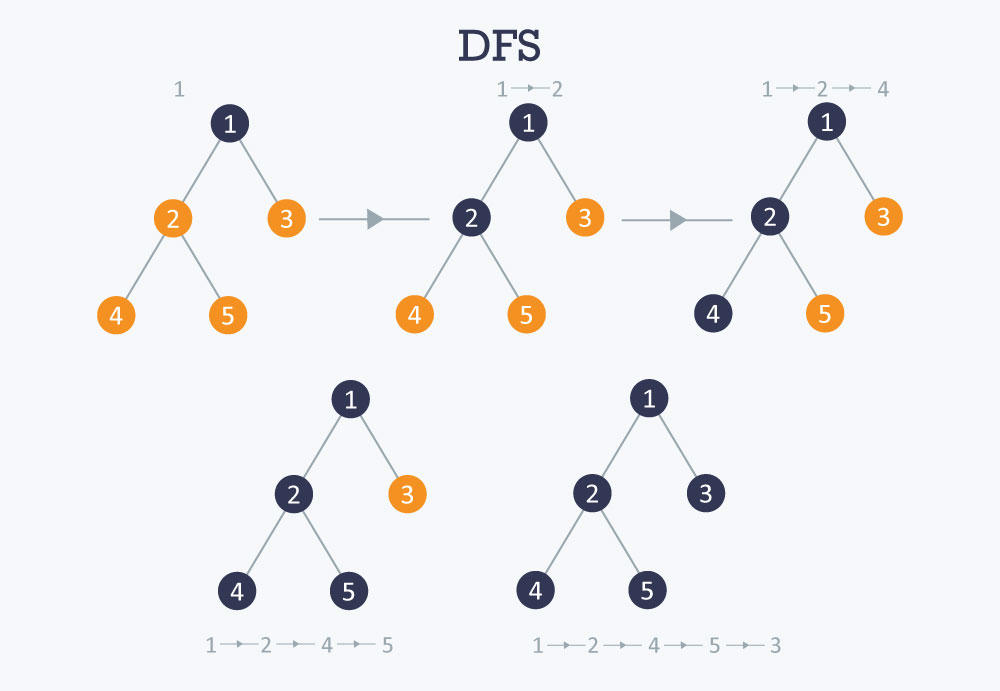
\includegraphics[width=.7 \textwidth]{GrafDFS.png}
    
    \caption{\emph{Figura 12: Exemple de DFS. Font: \url{https://www.hackerearth.com/practice/algorithms/graphs/depth-first-search/tutorial/}}}
\end{center}

A la figura 12, podem observar l'algorisme DFS en acció on els nodes negres representen nodes visitats i els taronges els no visitats, finalment tots acaben sent visitats. \newline

En els següents dos codis, considerem la implementació del DFS, primer utilitzant la recursió i seguidament utilitzant un $stack$ (pila).

\newpage

\begin{lstlisting}
// CODI DFS RECURSIÓ

vector<vector> adjacents; // Aquí guardem el graf
vector visitats; // Aquí guardem els nodes visitats

void DFS(int node){
    visitats[node] = true; // El marquem com a visitat
    for (auto nodeAdjacent : adjacents[node]) //Mirem nodes adjacents
        if (visitats[nodeAdjacent] == false) //Si no l'hem visitat
            DFS(nodeAdjacent); //Fem DFS amb el node adjacent
}

int main(){
    DFS(1); // Prenem el node 1 com a inicial
    
    for (int i = 0; i < n; i++)
        if (visitats[i] == true)
            cout << i << " "; // Imprimim tots els nodes visitats
}
\end{lstlisting}

\begin{lstlisting}
// CODI DFS PILA

vector<vector> adjacents; // Aquí guardem el graf
vector visitats; // Aquí guardem els nodes visitats

void DFS(){
    stack<int> pila;
    pila.push(1); // Prenem el node 1 com a inicial
    
    while (!pila.empty()){ // Mentres que puguem visitar nodes
        int node = pila.top(); // Agafem el node de dalt de la pila
        pila.pop(); // Traiem el node de la pila
        visitats[node] = true; // El marquem com a visitat
        for (auto nodeAdjacent : adjacents[node]) // Mirem nodes adjacents
            if (visitats[nodeAdjacent] == false) // Si no l'hem visitat
                pila.push(nodeAdjacent); // Afegim el node a la cua
    }
}

int main(){
    DFS();
    
    for (int i = 0; i < n; i++)
        if (visitats[i] == true)
            cout << i << " "; // Imprimim tots els nodes visitats
}

\end{lstlisting}
\newpage

En l'algorisme DFS primer es declaren els dos vectors essencials en els problemes de grafs: un vector d'adjacència (adjacents) on s'emmagatzema tots els nodes veïns o adjacents de cada node, un vector de nodes visitats (visitats) on es guarda el número de tots els nodes que ja s'han visitat per tal que un mateix node no sigui visitat infinitament i el programa acabi en un bucle sense fi.

Primerament, llegim el node inicial i l'afegim a la pila, per assegurar-nos que es visitin tots els nodes que es poden visitar a partir del node inicial, es declara en bucle que no pararà fins que la pila estigui completament buida, a cada pas del bucle s'agafa el node de sobre la pila, s'elimina d'aquesta i es marca com a visitat en el vector visitat, seguidament mitjançant un bucle s'agafen tots els veïns del node en el qual ens trobem i si no han estat visitats, els afegim a sobre la pila, finalment tots els nodes que podíem visitar ja han estat visitats i els imprimim.

L'algorisme DFS sempre forma un camí fins que arriba a un node en el qual tots els seus veïns ja han estat visitats gràcies a l'estructura de dades pila, ja que quan li afegim un altre node, aquest queda a sobre de tota la pila i, per tant, el següent pas del bucle serà des d'aquest node a causa del fet que sempre agafem el node que està a sobre de tota la pila.

Per entendre-ho millor, amb el següent graf (figura 13, faré una representació de com actuaria el DFS en aquest cas, en cada pas mostraré com seria la pila (la dreta representa el principi de la pila) i quins serien els nodes visitats.

\begin{center}
    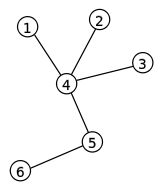
\includegraphics[width=.4 \textwidth]{tree.png}
    
    \caption{\emph{Figura 13: Graf (arbre). Font: \url{https://en.wikipedia.org/wiki/Tree_(graph_theory)}}}
\end{center}

Començarem per exemple pel node 1, l'afegim al començament de la pila. \newline

\textbf{Pila} [1]

\textbf{Visitat} [] \newline

Traiem el node 1 de la pila, l'afegim al vector visitat, mirem els seus nodes adjacents, afegim al començament de la pila el node 4. \newline

\textbf{Pila} [4]

\textbf{Visitat} [1] \newline

Traiem el node 4 de la pila, l'afegim al vector visitat, mirem els nodes adjacents al node 4, afegim els nodes 2, 3 i 5 al començament de la pila. \newline

\textbf{Pila} [2, 3, 5]

\textbf{Visitat} [1, 4] \newline

Traiem el node 5 de la pila, l'afegim al vector visitat, mirem els nodes adjacents al node 5, afegim al començament de la pila el node 6 i al vector visitats. \newline

\textbf{Pila} [2, 3, 6]

\textbf{Visitat} [1, 4, 5] \newline

Traiem el node 6 de la pila, l'afegim al vector visitat, mirem els nodes adjacents al node 6, no afegim cap node a la pila, ja que el seu node adjacent (5) ja ha estat visitat. \newline

\textbf{Pila} [2, 3]

\textbf{Visitat} [1, 4, 5, 6] \newline

Traiem el node 3 de la pila, l'afegim al vector visitat, mirem els nodes adjacents al node 3, no afegim cap node a la pila, ja que el seu node adjacent (4) ja ha estat visitat. \newline

\textbf{Pila} [2]

\textbf{Visitat} [1, 4, 5, 6, 3] \newline

Traiem el node 2 de la pila, l'afegim al vector visitat, mirem els nodes adjacents al node 2, no afegim cap node a la pila, ja que el seu node adjacent (4) ja ha estat visitat. \newline

\textbf{Pila} []

\textbf{Visitat} [1, 4, 5, 6, 3, 2] \newline

Com que la pila està buida, vol dir que ja hem visitat tots els nodes que podíem visitar i, per tant, el DFS finalitza.

